\begin{frame}
\frametitle{(Content Warning) Proof Culture in Machine Learning}
\pause
\begin{tikzpicture}
\node at (0,0) {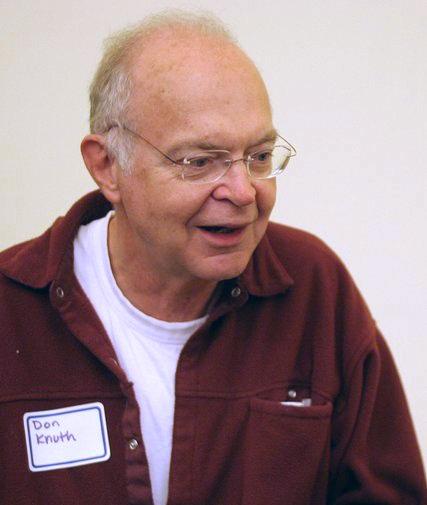
\includegraphics[width=2in]{img/knuth}};
\node at (6,0) {\parbox{2.4in}{
    \Large
Beware of bugs in the above code; I have only proved it correct, not tried it.

\vspace{0.2in}
-- Donald Knuth
}};
\end{tikzpicture}
\end{frame}

%%%%%%%%%%%%%%%%%%%%%%%%%%%%%%%%%%%%%%%%%%%%%%%%%%%%%%%%%%%%%%%%%%%%%%%%%%%%%%%%

\begin{frame}
\frametitle{(Content Warning) Proof Culture in Machine Learning}

Google Scholar's most cited paper of 2020:\footnote{
    \tiny\url{https://www.natureindex.com/news-blog/google-scholar-reveals-most-influential-papers-research-citations-twenty-twenty}
}

\vspace{0.1in}

\includegraphics[width=\textwidth]{img/adam}

\pause
\citet{reddi2019convergence}
\begin{itemize}
\item
    Simple counter example to Adam paper's proofs
\item
    Provide a fixed, corrected algorithm AdamW
\item
    ``Only'' 1500 citations
\item
    Adam paper has $>60000$ citations since \citet{reddi2019convergence} published
\end{itemize}
\end{frame}

%%%%%%%%%%%%%%%%%%%%%%%%%%%%%%%%%%%%%%%%%%%%%%%%%%%%%%%%%%%%%%%%%%%%%%%%%%%%%%%%

\begin{frame}
\frametitle{(Content Warning) Proof Culture in Machine Learning}

\begin{tikzpicture}
\node at (0,0) {
\includegraphics[width=2in]{img/facebookanon}};
\node at (6,0) {\parbox{2.4in}{
\begin{flushleft}
\Large
I don't care about theorems or proofs.
I only look at the experiments.

\vspace{0.2in}
-- Reviewer \#3
\end{flushleft}
}};

%\pause
    %\draw[red, line width=2pt] (3,0) -- (5.5,0);
    %\node at (7,-0.1) {\Large\color{red} cute animals};
\end{tikzpicture}

\end{frame}
